

\chapter{Noise Reduction through De-Whitening Filter}

\section{Concept of De-Whitening Filter}
Consider a situation in which the Photon Calibrator received white, frequency independent, excitation signal noise, it will generate $1/f^2$ displacement noise on End-Test-Mirror because the force to displacement transfer function contains $1/f^2$ feature. If we put an analog filter that has frequency response proportional to $f^2$ between excitation signal and PCal excitation input port, we may create colored, $f^2$, laser intensity noise from white electrical noise of excitation signal. Then, such colored noise will be whitened by $1/f^2$ force to displacement transfer function. We call the $f^2$ analog filter \emph{De-Whitening filter }


Practically, we use a one pole one zero analog filter with transfer function described in (ref) as our De-Whitening filter. 


\section{Circuit Design}
The main circuit design is described in Fig.~\ref{fig:dewcircuit}. The pole and zero frequency is determined by resistors and capacitors between A and B. We use 0.01$\mu$F Mica capacitor(CD30FD103FO3F made by Cornell Dubilier Electronics), whose capacitance tolerance is within 1\% and capacitance drift is within $\pm(0.05\% +0.1 pF)$ to reduce filter shape uncertainty caused by pole-zero frequency drifting.

The Transfer function of this circuit is
%\begin{equation}
%    \frac{(1+ i \omega R_b C)}{(1+\frac{R_b}{R_a}) + (i \omega R_b C )}
%\end{equation}

\begin{equation}
\label{eq:dewtf}
    \mathrm{DewTF} = \underbrace{\frac{Z_A}{Z_A+Z_B}}_{\text{pole-zero stage}} \times \underbrace{2}_{\text{Single to Differential}}
\end{equation}


where
\begin{align}
    A//B &\equiv \frac{1}{\frac{1}{A}+\frac{1}{B}} \\
    Z_B &= ( R_3 + \frac{1}{i \omega C_2} )~ //~ R_b \\
    Z_A &= ( R_4 + \frac{1}{i \omega C_1} )~ //~ R_a
\end{align}

When $R_3=R_4=a$, $C1=C2=C$, Eq.~(\ref{eq:dewtf}) will reduce to 

\begin{equation}
%\label{eq:dewtf}
    \mathrm{DewTF} = \frac{1+i \omega C (a+ R_b)}{1+\frac{R_b}{R_a} + i \omega C (2 R_b + a(1+\frac{R_b}{R_a}))}
\end{equation}

Practically, we will choose $a=100\Omega << R_a =8.37\mathrm{k}\Omega < R_b =159\mathrm{k}\Omega $ For DC, the gain is 
\begin{equation}
%\label{eq:dewtf}
    \mathrm{DewTF}\ \rvert_{\omega=0} = \frac{1}{1+\frac{R_b}{R_a}}
\end{equation}



%\begin{figure}[hbt!]
%\centering
\begin{sidewaysfigure}
%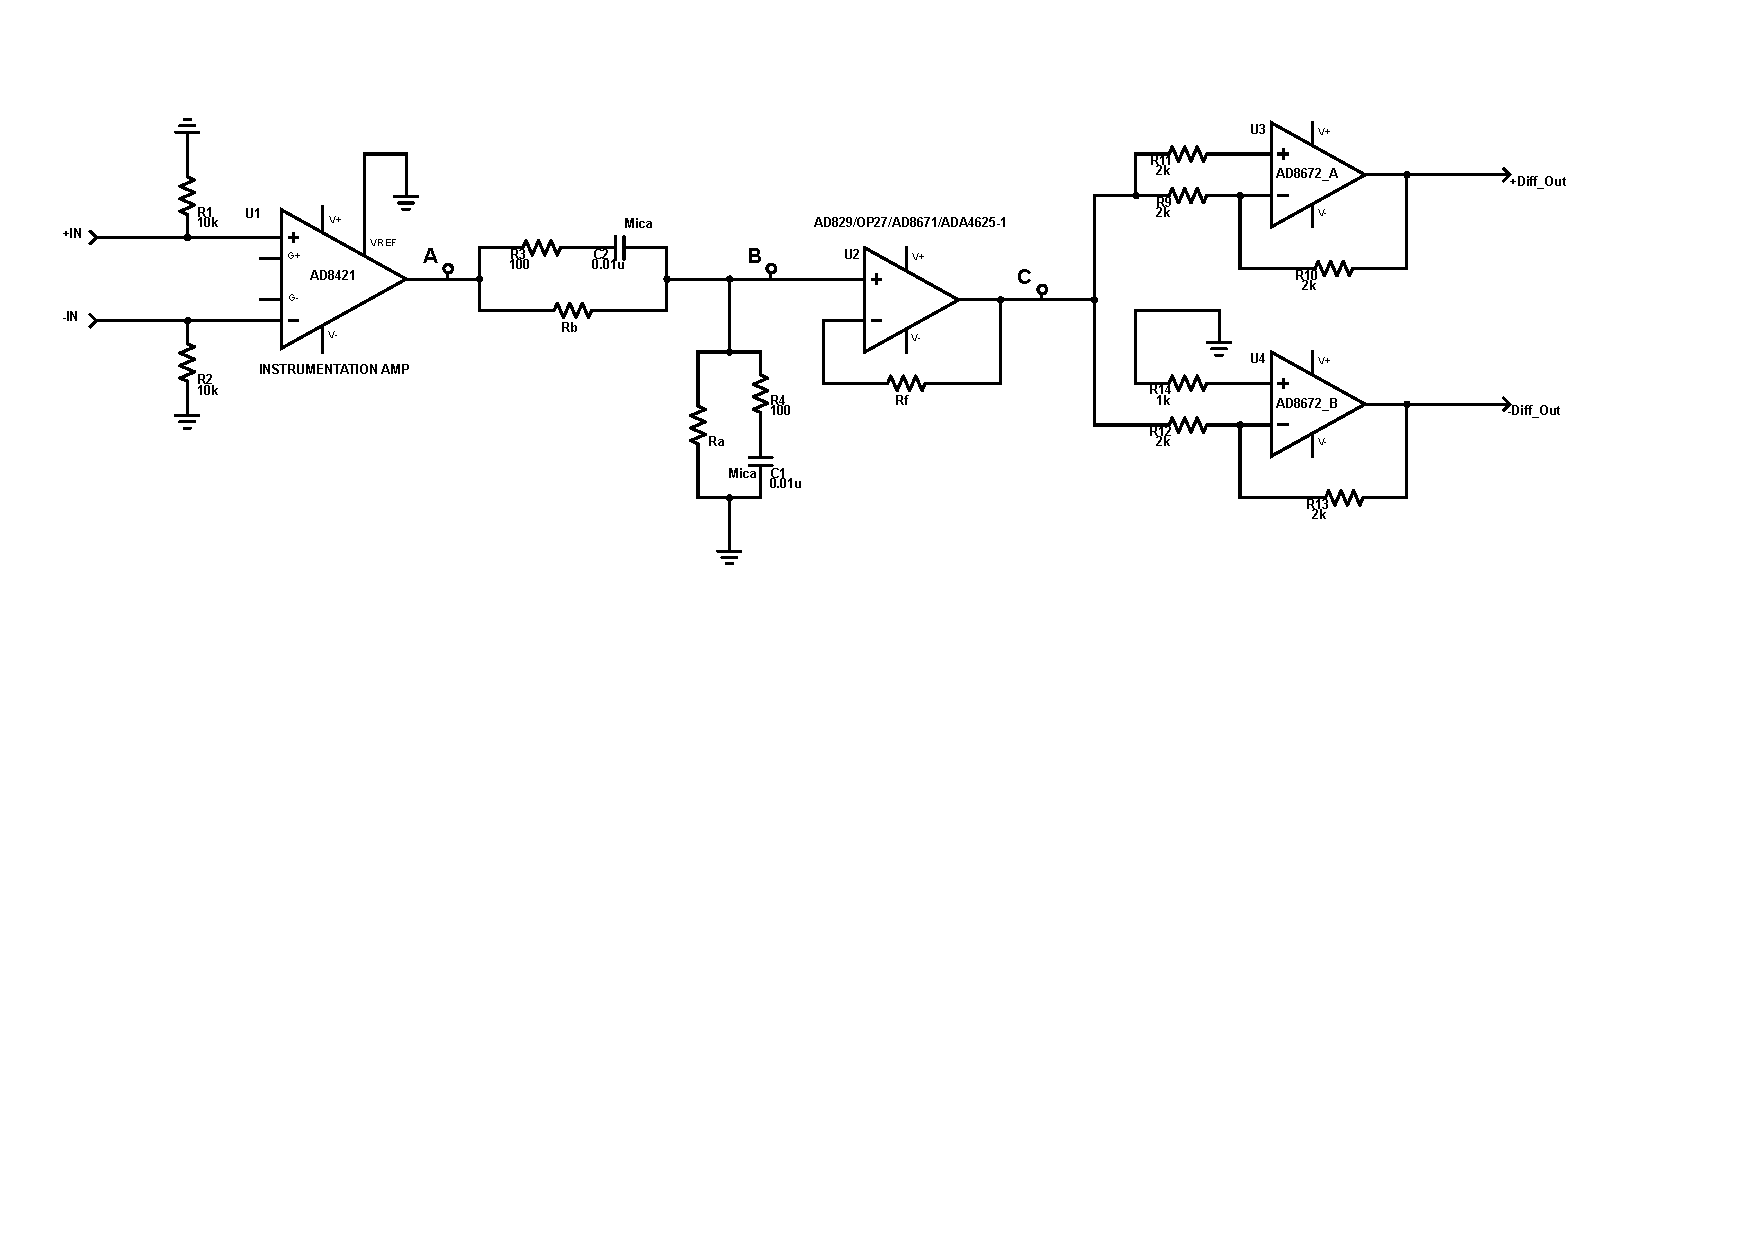
\includegraphics[angle=90, width=0.48\textwidth]{figure/DEWcircuit.pdf}
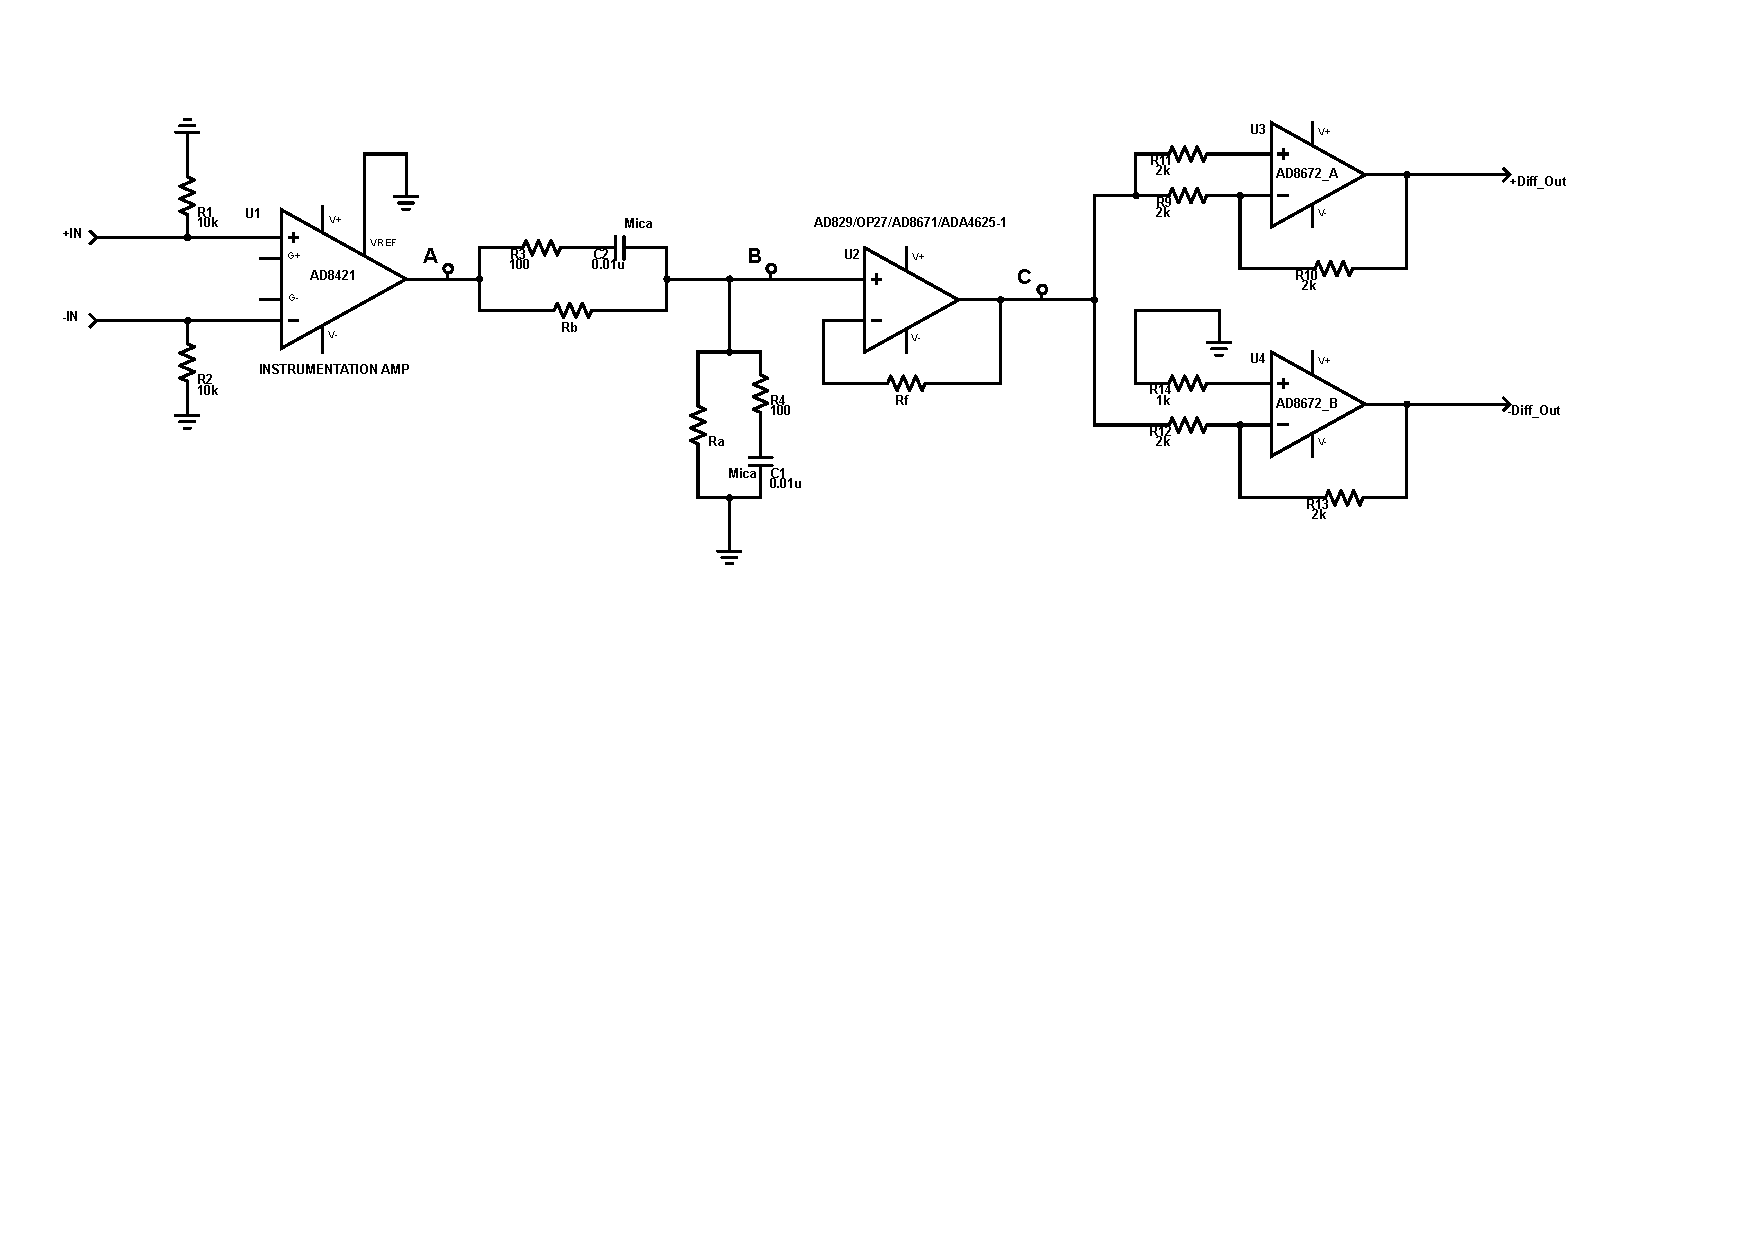
\includegraphics[width=1\textwidth]{figure/DEWcircuit.pdf}
\caption[De-Whitening filter circuit]{De-Whitening filter circuit. There are three points labeled as A, B,and C in the diagram. Before A, the differential input signal provided by Digital System will be converted into single single by a instrumentation amplifier AD8421. After that, a passive pole zero stage between A and B defines the dominate transfer function of De-Whitening filter. Then we put a voltage follower between B and C as a buffer to keep passive filter response. Finally, we convert signal back to differential signal to match downstream device input. }\label{fig:dewcircuit}
\index{figures}
\end{sidewaysfigure}
%\end{figure}



\section{Fidelity of Injection Signal}
%\subsection{Transfer Function of De-Whitening Filter}
The fidelity of injected signal is the fundamental requirement of hardware injection test. One can estimate the distortion of injected waveforms by measuring transfer function between excitation port in the software and PCal laser intensity. With De-Whitening filter, although we 

\begin{figure}[bt]
\centering
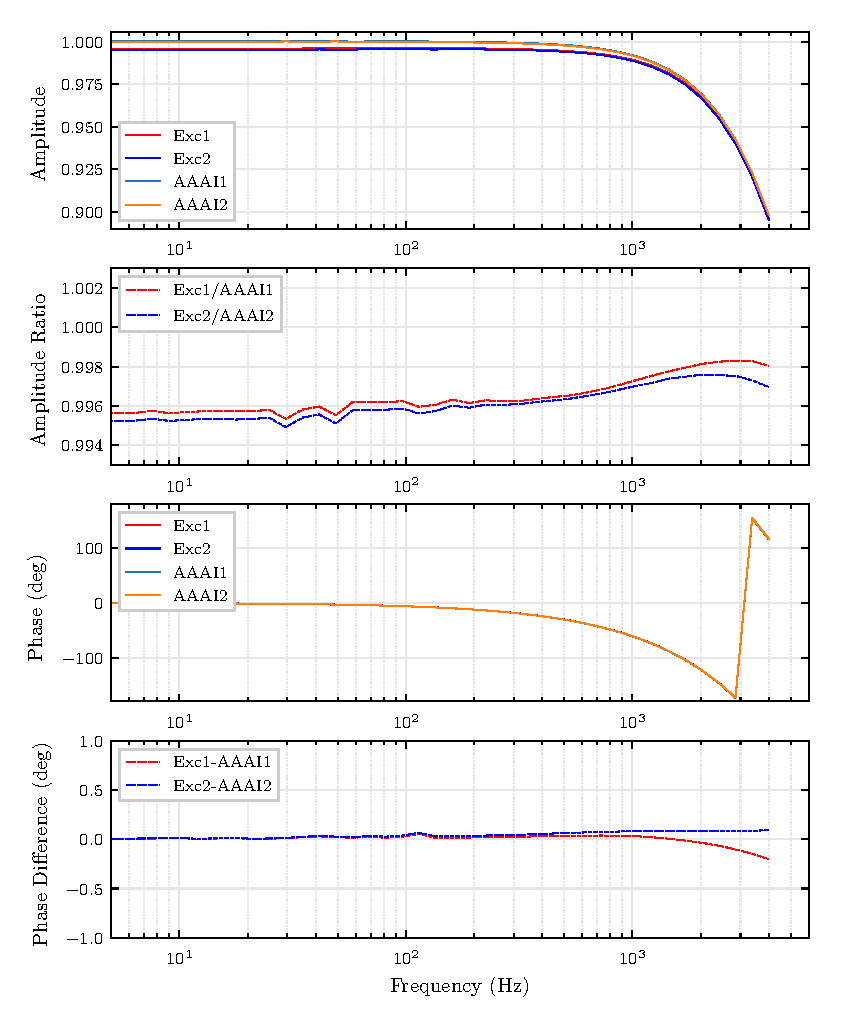
\includegraphics[width=1\textwidth]{figure/tf/TF_KEK_64}
\caption[Transfer function of De-Whitening Filter with Digital Inverse Filter]{Transfer function of De-Whitening Filter with Digital Inverse Filter. The transfer function is measured in KEK cryogenic center with KAGRA standalone digital system and 64kHz salve model.}\label{fig:tf64}
\index{figures}
\end{figure}
%\subsection{Transfer function of Digital Inverse Filter}


\section{Noise Reduction Performance}
In principle, a 

\begin{figure}[bt]
\centering
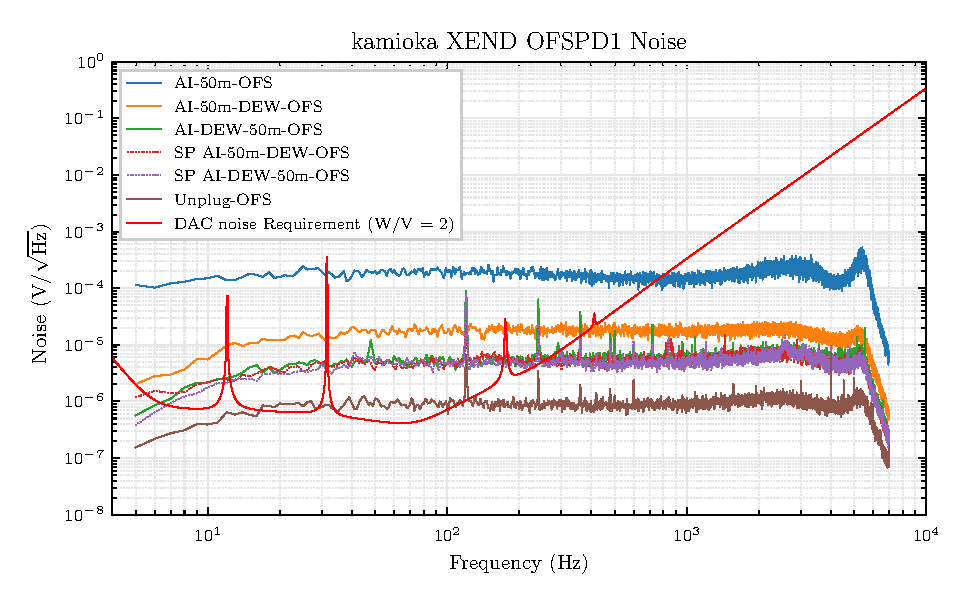
\includegraphics[width=1\textwidth]{figure/noise/DEWnoiseKamiokaSP}
\caption{Noise}\label{fig:noiseKSP}
\index{figures}

\end{figure}
\begin{figure}[bt]
\centering
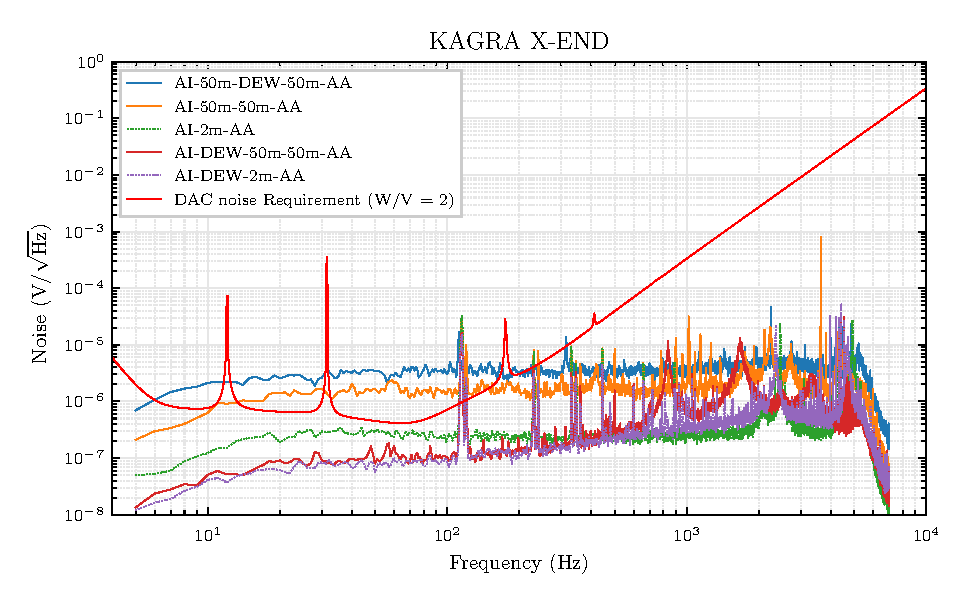
\includegraphics[width=1\textwidth]{figure/noise/DEWnoiseKamioka}
\caption{Noise}\label{fig:noiseK}
\index{figures}
\end{figure}